%\documentclass[11pt,a4paper]{book}
\documentclass[a4paper,openright,12pt,noshorthands,spanish]{book}

% Cargar preámbulo
% Preámbulo general
\usepackage[utf8]{inputenc}
\usepackage[T1]{fontenc}
\usepackage{geometry}
\geometry{a4paper, margin=1in}
\usepackage{graphicx}
\usepackage{hyperref}
\usepackage{xcolor}
\usepackage{mathpazo} % Fuente Palatino para texto
\usepackage[scaled=0.9]{helvet} % Helvética para títulos


% Opciones adicionales
\usepackage{titlesec}
\titleformat{\section}{\Large\bfseries}{\thesection.}{0.5em}{}

\renewcommand{\contentsname}{Contenido}

\newcommand{\titlepageAMS}{
  \begin{titlepage}
    \centering
    \vspace*{2cm}
    {\Huge\bfseries \textsf{Compendio de la Teoría de los Números}}\\[1cm]
    {\Large\bfseries \textsf{César A. Díaz M.}}\\[3cm]
    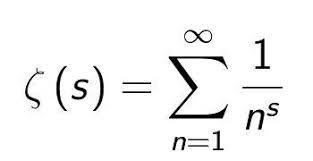
\includegraphics[width=0.3\textwidth]{images/logo_1.jpg}\\[2cm]
    {\large \textit{Publicación independiente}}\\[0.5cm]
    {\large \textit{\today}}\\[5cm]
    \textsf{Con el apoyo de la comunidad matemática}\\[1cm]
    \vfill
  \end{titlepage}
}


\begin{document}

\titlepageAMS
% Página en blanco después de la portada
\newpage\thispagestyle{empty}\mbox{}\newpage

% Tabla de contenido
\tableofcontents
\newpage

% Índices y prefacios
\frontmatter
\chapter*{Índice Alfabético}
\addcontentsline{toc}{chapter}{Índice Alfabético}

%\phantomsection
%\cleardoublepage
%\addcontentsline{toc}{chapter}{\indexname}
%\clearpage
%\addcontentsline{toc}{}{}
\printindex
%\addcontentsline{toc}{chapter}{\indexname}       % Índice (puede generarse con `makeindex`)
\newglossaryentry{conjunto}{
    name=Conjunto,
    description={Una colección de elementos}
}

\newglossaryentry{teorema}{
    name=Teorema,
    description={Un enunciado demostrable en matemáticas}
}

\newglossaryentry{supremo}{
    name=Supremo,
    description={El menor límite superior de un conjunto}
}

%\chapter*{Glosario}
%\addcontentsline{toc}{chapter}{Glosario} % Añade el glosario al índice de contenidos
\printglossaries
    % Glosario de términos

% Contenido principal
\mainmatter
\chapter{Combinatoria Aditiva}
Este capítulo es un compendio de resultados en combinatoria aditiva.

% Incluir secciones del capítulo
\section{Densidad de Schnirelmann}
Sea $A\subset \N_0 = \set{0,1,2,3,\ldots}$. La densidad de Schnirelmann del conjunto $A$ se denota y se define como 
\begin{equation}
    \sigma(A) = \inf_{n\geq 1} \set{\frac{\abs{\set{1,2,3,\ldots,n}\cap A}}{n}}
\end{equation}

%Ejemplo de cita: Como se menciona en \cite{hardy2008numbers}, los números primos son fundamentales.
%\input{chapters/chapter1/section2}
%\input{chapters/chapter1/section3}

\chapter{Teorema de Roth}
Usar indices: \index{Al índice} k

% Apéndices
\appendix
\chapter{Demostraciones Adicionales}

\section{Demostración del TFC}
Aquí puedes agregar demostraciones adicionales.

\chapter{Pruebas de newcommands, index, glossary, etc}

Este es el capítulo 1 de tu libro de matemáticas.

\section{Ejemplo de Teorema}

\begin{theo}[Pitagoras]
En un triángulo rectángulo, el cuadrado de la hipotenusa es igual a la suma de los cuadrados de los catetos.
\end{theo}

\begin{dem}
Sea un triángulo con lados $a$, $b$ y $c$, donde $c$ es la hipotenusa. Según el Teorema de Pitágoras:
\[
c^2 = a^2 + b^2.
\]
\end{dem}

\begin{afir}
Esta es una afirmación.
\end{afir}

\begin{obs}
    Esta es una observación
\end{obs}

\begin{defi}
Esta es una definición
\end{defi}

\begin{lemma}
    Este es un lema.
\end{lemma}

\begin{corol}
    Este es un corolario valor absoluto: $\abs{x}$, norma: $\norm{x}$, 
    conjunto $$A=\set{a_1,a_2,a_3}$$
\end{corol}

\begin{ejem}
    Este es un ejemplo
\end{ejem}
\section{Ejemplo de índice}
Este es un ejemplo de cómo usar el comando \index{Teorema} para generar índices.
\section{Ejemplo de glosario}
\begin{theo}
Este teorema es importante.\index{Teorema!Importante}
\end{theo}

Un \gls{teorema} es un concepto fundamental.

% Bibliografía
\backmatter
\bibliographystyle{amsplain}  % Estilo AMS para bibliografías
\nocite{*} % Agrega el contentido completo de references.bib (si se comenta se agrega solo las referencias citadas)
\bibliography{references}

\end{document}
